\setchapterpreamble[u]{\margintoc}
\glsresetall % reset glossary
\chapter{Evaluating discretization approaches for ultralight structure optimization}
\todo{check buchi fatti dallo spostamento}
The process of topology optimization for a structure involves the selection and sizing of optimal elements within a predetermined set. As discussed in the previous chapter, in our context this set could be composed of either continuum elements (shell or volumetric) or truss-like elements. This chapter aims to assess the suitability and the inherent advantages and disadvantages of both methodologies when optimizing ultralight structures \ie structures that exhibit \marginnote{Part of the content presented in this chapter has been published and showcased during a conference as:\\Stragiotti, E. et al. (2021) "Towards manufactured lattice structures: a comparison between layout and topology optimization", in \textit{AeroBest 2021 International Conference on Multidisciplinary Design Optimization of Aerospace Systems}. Book of proceedings. Lisbon, Portugal: ECCOMAS~\cite{stragiotti_towards_2021}.} an extremely low volume fraction, typically below 1\%. 

For this purpose, we initially establish a common optimization formulation in \secref{sec:03_common_prob}. The classic compliance minimization with volume constraint problem is reformulated as a volume minimization problem with maximum stress constraints for both discretizations. Later, this framework is applied to optimize a two-dimensional test case, featuring identical dimensions, loads, and material properties. The outcomes of the comparison of both discretization approaches are presented and discussed in \secref{sec:03_comparison}. 

\section{The formulation of a common problem: volume minimization with stress constraints} \label{sec:03_common_prob}
Two of the most frequently employed formulations for structural optimization are the minimization of volume while adhering to stress constraints and the minimization of compliance under volume constraints. Historically, the volume minimization formulation has been used in the first works of structural optimization of truss structures~\sidecite{dorn_automatic_1964,chan_optimum_1964,hemp_optimum_1973}. The problem was initially formulated in terms of member forces, ignoring the kinematic compatibility to obtain a \gls{lp} problem. The formulation was modeled using the \acrfull{sand} approach, where the equations of nodal equilibrium are treated as equality constraints, and where both nodal displacements and the cross-sectional areas of truss members serve as design variables~\sidecite{sankaranarayanan_truss_1994}. 

However, to attain greater design freedom, the structure optimization field later transitioned from truss structures to continuous discretization. While truss structures offered simplicity and ease of analysis, they imposed limitations on design due to their discrete member configurations. The continuum mesh offered instead more versatility~\sidecite{bendsoe_generating_1988,bendsoe_optimal_1989}, and has since been used for multiple different applications, \eg the design of metamaterials~\sidecite{sigmund_materials_1994, zhang_scale-related_2006} or the simulation of advanced manufacturing constaints~\sidecite{sigmund_manufacturing_2009,brackett_topology_2011}. The \gls{sand} approach is incompatible with continuum meshes due to its excessive number of variables\sidenote{This preposition holds when referring to the end of the 1980s when computational power was scarce compared to what we have today.}. Given this limitation, a new approach was required to better handle the complexity of continuum meshes.

In the \acrfull{nand} approach, the nodal displacement (state) variables are eliminated from the optimization problem through a process where the structural equilibrium equation is solved every iteration instead of being used as a constraint of the optimization. This results in an independent nested phase where the state equation of structural equilibrium is solved separately from the optimization algorithm. This creates a dense coupling between displacement and material density variables, necessitating a computationally expensive sensitivity analysis within the nested algorithm, typically employing the adjoint method (more information about the adjoint method on the following resurces~\sidecite{tortorelli_design_1994,martins_engineering_2021}). Nevertheless, if the problem is reformulated as a compliance minimization with volume constraints, the problem is self-adjoint and the adjoint algorithm is no longer necessary to evaluate the gradient sensitivities~\sidecite{bendsoe_topology_2004}.

However, our emphasis on operating within the aerospace sector aligns more favorably with the volume minimization problem. The choice to prioritize volume minimization in the aerospace sector is underpinned by a range of economic, environmental, and performance-related factors. It is a strategic approach that aligns with industry goals of sustainability, efficiency, and technological advancement. Additionally, as we will see later in this thesis, the volume minimization formulation will permit adding local buckling and maximum displacement constraints more easily. We have opted, thus, to employ the volume minimization optimization formulation for our study, and we will now review how this formulation is implemented on continuum and truss-like meshes.

\subsection{Continuous discretization \gls{nand} minimum volume formulation}
This section introduces the \gls{nand} volume minimization formulation of topology optimization for continuum meshes. We will start however presenting the more common minimum compliance formulation to explain the important notations and concepts that will be essential in developing the volume minimization formulation.
\todo{modify here}
\paragraph{Objective and constraint functions}
Up until this point, we have been focused on the compliance minimization formulation \eqrefnotext{eq:03_prob-comp}. Moving forward, we introduce the necessary modifications to transition into the volume minimization formulation with stress constraints. This formulation will be used to compare the continuous mesh with truss-like structure optimization.

The objective of the optimization is to minimize the volume of a structure subject to a specified load case. The volume of the structure $V$ is expressed as a fraction of the total volume $V_0$ of the domain $\Omega$:
\begin{equation}
    V = \frac{1}{V_0}\sum_{i \in \Omega} \rhophys_i v_i.
    \label{eq:03_vol_v}
\end{equation}
In this thesis, we assume that the elementary volume occupied by the $i$-th element $v_i$ is equal for all the elements, and thus \eqref{eq:03_vol_v} is simplified as follows:
\begin{equation}
    V = \frac{1}{N_{e}} \sum_{i \in \Omega} \rhophys_i. 
    \label{eq:03_obj_vol}  
\end{equation}
The normalized local stress constraint $\vect{g}_{\text{st}}$ are formulated as:
\begin{equation}
    \frac{\sigma_{\text{VM},i}}{\sigma_L}-1 \leq 0, \quad \forall i \in \Omega_{mat}(\bm{\rho})
    \tag{$g_{\text{st}}$}
\end{equation}
where $\Omega_{mat}(\bm{\rho}) \subseteq \Omega$ represents the design-dependent set of elements with a non-zero density, $\sigma_{\text{VM},i}$ is the equivalent Von Mises stress for the $i$-th element, and $\sigma_L$ is the maximum allowable of the material.

The first difficulty that arises is that the stress constraints are defined only for the elements where $\rhophys_i > 0$, while $\rhophys_i\in[0,1]$. Thus, the set of constraints changes during the optimization. This class of problems is called \acrfull{mpvc}~\sidecite{achtziger_mathematical_2008} and is known for being difficult to solve with a gradient descent optimization algorithm. The original set of constraints $\vect{g}_{\text{st}}$ is then reformulated into an equivalent design-independent set of constraints $\bar{\vect{g}}_{\text{st}}$ as follows~\sidecite{cheng_study_1992}:
\begin{equation}
    \rhophys_i\left(\frac{ \sigma_{\text{VM},i}}{\sigma_L}-1 \right) \leq 0, \quad \forall i \in \Omega.
    \tag{$\bar{g}_{\text{st}}$}
\end{equation}
\paragraph{Von Mises stress evaluation}
The evaluation of the equivalent stress of an element follows the formulation proposed by Von Mises. Let us take a four-node quadrilateral linear element with a single integration (or Gauss) point in the center and four $2a$ equal-length sides (see \figref{fig:03_gp}). If bilinear shape functions are used to interpolate the displacement field, we can evaluate the deformations at the integration point as:
\begin{equation}
    \begin{pmatrix}
    \varepsilon_\text{x} \\
    \varepsilon_\text{y} \\
    \gamma_{xy}
    \end{pmatrix} = \matr{B}_s\vect{q}_s
    \textrm{,  with }
    \matr{B}_s =
    \frac{1}{4a}
    \begin{pmatrix}
    -1  &   1   &   1   &   -1  &   0   &   0   &   0   &   0   \\
    0   &   0   &   0   &   0   &   -1  &   -1  &   1   &   1   \\
    -1  &   -1  &   1   &   1   &   -1  &   1   &   1   &   -1
    \end{pmatrix},
\end{equation}
where $\vect{q}_s = (u_1, u_2, u_3, u_4, v_1, v_2, v_3, v_4)^T$ represents the vector of the displacement degrees of freedom of the element. 

\begin{marginfigure}
    \centering
    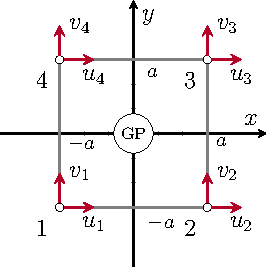
\includegraphics{figures/03_comparison_TO_TTO/03_gauss_point/gp.pdf}
    \caption{A four-node quadrilateral element. GP is the Gaussian integration point for which the equivalent stress is evaluated.}
    \label{fig:03_gp}
\end{marginfigure}


The stress tensor is evaluated using the elasticity Hooke's law in 2D as follows: 
\begin{equation}
    \begin{pmatrix}
    \sigma_x \\
    \sigma_y \\
    \tau_{xy}
    \end{pmatrix}
    =\matr{C}_e
    \begin{pmatrix}
    \varepsilon_\text{x} \\
    \varepsilon_\text{y} \\
    \gamma_{xy}
%     \end{pmatrix},
%     \quad
%    \text{with }
    \end{pmatrix}
    \quad
    \text{with}
    \quad
    \matr{C}_e = \frac{E}{1-\nu^2}
    \begin{pmatrix}
    1   &   \nu &   0   \\
    \nu &   1   &   0   \\
    0   &   0   &   G
    \end{pmatrix}.
\end{equation}

The equivalent Von Mises stress of the element can then be written as:
\begin{align}
    \langle \vect{\sigma}_{\text{VM}} \rangle &= \sqrt{\sigma_x^2 + \sigma_y^2 - \sigma_x \sigma_y+3\tau_{xy}} \\
    &= \sqrt{
    \begin{pmatrix}
    \sigma_x & \sigma_y & \tau_{xy}
    \end{pmatrix}
    \begin{pmatrix}
    1       &   -1/2    &   0   \\
    -1/2    &   1       &   0   \\
    0       &   0       &   3
    \end{pmatrix}
    \begin{pmatrix}
    \sigma_x \\
    \sigma_y \\
    \tau_{xy}
    \end{pmatrix}} \\
    &= \sqrt{\vect{q}_s^T\matr{B}_s^T\matr{C}_e^T\matr{D}_{\text{VM}}\matr{C}_e\matr{B}_s\vect{q}_s}
    \textrm{,  with } \matr{D}_{\text{VM}} = 
    \begin{pmatrix}
    1       &   -1/2    &   0   \\
    -1/2    &   1       &   0   \\
    0       &   0       &   3
    \end{pmatrix} \\
    \langle \vect{\sigma}_{\text{VM}} \rangle &= \sqrt{\vect{q}_s^T\matr{S}\vect{q}_s}, \quad
    \textrm{with } \matr{S} = \matr{B}_s^T\matr{C}_e^T\matr{D}_{\text{VM}}\matr{C}_e\matr{B}_s.
    \label{eq:03_VM_calc}
\end{align}
\paragraph{Microscopic and macroscopic stress}
In stress-constrained topology optimization, the element stress is usually evaluated using the microscopic stress formulation, assuming that there is no direct correlation between stress and density~\sidecite{duysinx_topology_1998}. Indeed, the use of the macroscopic stress in volume minimization optimization problems creates an all-void design~\sidecite{le_stress-based_2010}. The properties that the microscopic stress should present are:
\begin{enumerate}[label=(\roman*)]
    \item The stress criterion should be mathematically as simple as possible, as the relationship between Young's modulus and density. This permits a simple numerical implementation.
    \item To mimic the real physical behavior, the microscopic stress should be inversely proportional to density.
    \item The microscopic stress should converge to a non-zero value at zero density. This requisite is deduced from investigations into the asymptotic stress behavior in thin layers~\sidecite{verbart_unified_2017}.
\end{enumerate}

The relation between stress and displacement is written as:
\begin{equation}
    \langle \vect{\sigma}_{\text{VM}} \rangle = \matr{C}_e(\langle E \rangle) \langle \vect{\varepsilon} \rangle,
    \label{eq:03_stress_disp}
\end{equation}
where the variables between angular brackets $\langle \dots \rangle$ represent macroscopic variables.

Combining (i) and (ii) with \eqsref{eq:03_simp} and \eqrefnotext{eq:03_stress_disp}, the microscopic stress can be written as:
\begin{equation}
    \vect{\sigma}_{\text{VM}} = \frac{\langle \vect{\sigma}_{\text{VM}} \rangle}{\rho^q_e} = \rho_e^{p-q} \matr{C}_e(E_0)\langle \vect{\varepsilon} \rangle,
\end{equation}
where the exponent $q$ is a number greater than 1.

One possible choice that satisfy all the requirements is $q=p$~\sidecite{le_stress-based_2010,verbart_unified_2017,holmberg_stress_2013,da_silva_stress-constrained_2019}. Thus, the microscopic stress is defined as:
\begin{equation}
    \vect{\sigma}_{\text{VM}} = \matr{C}_e(E_0)\langle \vect{\varepsilon} \rangle.
    \label{eq:03_micro_stress}
\end{equation}
From a physical perspective, the significance of microscopic stress becomes evident when considering an element with intermediate density and a porous microstructure. The microscopic stress presented in \eqref{eq:03_micro_stress} measures the stress of the microstructure. It is grounded in the assumption that the macroscopic deformations of the homogenized element generate within the microstructure of the element a stress state that remains unaffected by the density of the element itself.

\paragraph{Constraints aggregation and relaxation}
When optimizing a structure with stress constraints using a \gls{nand} formulation, two primary challenges commonly arise:
\begin{enumerate}[label=(\roman*)]
    \item Is it known in the literature \cite{rozvany_design-dependent_2001,stolpe_models_2003} that stress-based topology optimization suffers from the \textit{singular minima} (or \textit{singularity}) problem: firstly observed on truss structure optimization \cite{sved_structural_1968}, these \textit{minima} are almost inaccessible to a standard gradient-based optimizer, and they represent the \textit{minima} of the optimization. This is because achieving the optimal solution to a problem using continuous design variables may necessitate passing through a state where the optimization constraints are violated, \ie the \textit{minimum} is on a lower dimension compared to the design space. This problem is often solved using a technique called \textit{constraints relaxation}~\sidecite{cheng_relaxed_1997}.

    \item The stress is a local measure, and thus a large set of constraints is generated when a reasonably fine mesh is used (one element, one constraint). This problem is often solved using a technique called \textit{constraints aggregation} or \textit{global constraints}~\sidecite{da_silva_local_2021}.
\end{enumerate} 

Following the work developed by Verbart \etal~\sideciteonce{verbart_unified_2017}, the lower bound \gls{ks} function~\sidecite{kreisselmeier_systematic_1979} is used to approximate the local relaxed stress constraint maximum. The authors discovered that employing lower-bound \gls{ks} aggregation functions to approximate the maximum operator in stress-constrained topology optimization eliminates the need for stress constraint relaxation methods to address the singularity issue. This is because the lower-bound functions inherently offer a combined effect of constraint aggregation and relaxation. The \gls{ks} aggregated stress constraint function is defined as follows:
\begin{equation} 
    G_{\text{KS}}^\text{L} = \frac{1}{P} \ln{\left( \frac{1}{N_\text{e}} \sum e^{{P}\bar{g}_i} \right)}.
    \label{eq:03_gksl}
\end{equation}
Its main advantage over other different formulations is that it uses a single hyperparameter $P$ to control the aggregation and the relaxation of the constraints simultaneously.

\paragraph{Minimum volume formulation}
The \gls{nand} minimum volume formulation for continuous discretization is written combining \eqsref{eq:03_obj_vol} and \eqrefnotext{eq:03_gksl} as:
\begin{equation}
    \begin{aligned}
    \min_{\bm{\rho}}         && V &= \frac{1}{N_{e}} \sum_{i \in \Omega} \rhophys_i,  \\
    \textrm{s.t.}   && G_{\text{KS}}^\text{L} &= \frac{1}{P} \ln{\left( \frac{1}{N_\text{e}} \sum_{i \in \Omega} e^{{P}\bar{g}_i} \right)} \leq 0 \\
    && \bm{K}\bm{u} &= \bm{F}\\
    && 0 &\leq \rho_i \leq 1, \\
    \end{aligned}
    \tag{$\mathbb{T}_1$}
    \label{eq:03_prob-stress}
\end{equation}
The optimization is carried out using a gradient descent optimization algorithm for which the sensitivities are given in analytical form. Using analytic gradients is in general more efficient than finite differences as it avoids the need for multiple function evaluations, making the optimization process faster and more precise.

\paragraph{Sensitivity analysis of the objective function}
The objective of this section is to quickly present the calculation of the analytical sensitivity of the volume with respect to the design variable $\rho$. Deriving \eqref{eq:03_obj_vol} we obtain:

\begin{equation}
    \derfrac{V}{\rhophys_i} = \frac{1}{N_{e}}.
    \label{eq:03_01}
\end{equation}
The sensitivity of the objective function can then be evaluated using \eqsref{eq:03_01} \eqrefnotext{eq:03_sens_filt}, \eqrefnotext{eq:03_sens_proj}, and \eqrefnotext{eq:03_chain} as follows:
\begin{equation}
    \frac{d V}{d \rho_i} = \sum_{j \in \mathbb{N}_{i,R}} \derfrac{V}{\rhophys_j} \derfrac{\rhophys_j}{\rhofil_j} \derfrac{\rhofil_j}{\rho_i}.
\end{equation}
\paragraph{Sensitivity analysis of the constraint function}
This section focuses on the details of the calculation of how the constraint function $G_{\text{KS}}^\text{L}$ changes with respect to the design variable $\vect{\rho}$. The sensitivity of the aggregated constraint function with respect to the design variable $\vect{\rho}$ is evaluated using:
\begin{equation} \label{eq:03_chain_sens_fin}
    \frac{d G_{\text{KS}}^\text{L}}{d \rho_i} = \sum_{j \in \mathbb{N}_{i,R}} \derfrac{G_{\text{KS}}^\text{L}}{\rhophys_j} \derfrac{\rhophys_j}{\rhofil_j} \derfrac{\rhofil_j}{\rho_i}.
\end{equation}

As the constraint function $G_{\text{KS}}^\text{L} = G(\vect{\rhophys}, \vect{u}(\vect{\rhophys}) )$ is explicitly and implicitly (via the relationship with $\vect{u}$) depending on $\vect{\rhophys}$, the first-order derivative is evaluated using the total derivative formula:
\begin{equation} \label{eq:03_sens-0}
    \derfrac{G_{\text{KS}}^\text{L}}{\rhophys_j} = \frac{d G}{d \rhophys_j} = \derfrac{G}{ \rhophys_j} + \derfrac{G}{\vect{u}} \frac{d \vect{u} }{d \rhophys_j}.
\end{equation}
As function $G_{\text{KS}}^\text{L}$ depends on $\vect{u}$ via the stresses $\sigma_i$, it is possible to write:
\begin{equation} \label{eq:03_sens-1}
    \derfrac{G}{\vect{u}} = \sum_{i \in \Omega} \left( \derfrac{G}{\sigma_i} \derfrac{\sigma_i}{\vect{u}}\right).
\end{equation}
Combining Eq. \ref{eq:03_sens-0} with Eq. \ref{eq:03_sens-1}, we obtain:
\begin{equation} \label{eq:03_sens-2}
    \frac{d G}{d \rhophys_j} = \underbrace{\derfrac{G}{\rhophys_j}}_A + \sum_{i \in \Omega} \left( \underbrace{\derfrac{G}{\sigma_i}}_B \underbrace{\derfrac{\sigma_i}{\vect{u}}}_C \right)  \underbrace{\frac{d \vect{u} }{d \rhophys_j}}_D.
\end{equation}
We compute the four factors separately:
\begin{enumerate}[label=\Alph* --]
    \item The first term represents the explicit relationship of $G$ to the physical densities and its calculation is straightforward: 
    \begin{equation} \label{eq:03_sens-2-1}
        \derfrac{G}{ \rhophys_j} = \frac{1}{P} \frac{\left(\frac{ \sigma_{\text{VM},j}}{\sigma_L}-1 \right)\frac{1}{N_\text{e}} P e^{{P}\bar{g}_j}}{\frac{1}{N_\text{e}} \sum_k e^{{P}\bar{g}_k}} = \left(\frac{ \sigma_{\text{VM},j}}{\sigma_L}-1 \right) \frac{e^{{P}\bar{g}_j}}{\sum_k e^{{P}\bar{g}_k}}.
    \end{equation}
    
    \item The second term can be calculated using the chain rule:
    \begin{equation}
        \label{eq:03_sens-2-2}
        \derfrac{G}{\sigma_i} = \derfrac{G}{\bar{g}_i} \derfrac{\bar{g}_i}{\sigma_i} = \frac{1}{P} \frac{\frac{1}{N_\text{e}} P e^{{P}\bar{g}_i}}{\frac{1}{N_\text{e}} \sum_k e^{{P}\bar{g}_k}} \frac{\rhophys_i}{\sigma_L} = \frac{\rhophys_i}{\sigma_L} \frac{e^{{P}\bar{g}_i}}{\sum_k e^{{P}\bar{g}_k}}.
    \end{equation}
    
    \item We reformulate \eqref{eq:03_VM_calc} to be written in global coordinates instead of local:
    \begin{equation}
        \label{eq:03_sens-3}
        \sigma_i^2 = \vect{q}_s^T\matr{S}\vect{q}_s = \vect{u}^T |\matr{S_i}|_g \vect{u},
    \end{equation}  
    where $|\matr{S_i}|_g$ represents the matrix $\matr{S}$ of \eqref{eq:03_VM_calc}written on global coordinates \sidenote{The matrix $|\matr{S_i}|_g$ can be calculated using the very same assembling approach used for the stiffness matrix $\matr{K}$ starting from the elemental stiffness matrix $\matr{K}_e$. As the global stiffness matrix $\matr{K}$, $|\matr{S_i}|_g$ is symmetric and sparse.}. We can now differentiate \eqref{eq:03_sens-3} with respect of the displacement field in global coordinates $\vect{u}$ to obtain:
    \begin{equation}
        \label{eq:03_sens-4}
        \derfrac{\sigma_i}{\vect{u}} = \frac{|\matr{S_i}|_g \vect{u}}{\sigma_i}.
    \end{equation}
    \eqsref{eq:03_sens-2-2} and \eqrefnotext{eq:03_sens-4} are now combined to obtain the result of the product of the \textbf{B} and \textbf{C} terms. As a result, the derivatives of $G$ with respect to $\bm{u}$, are written as:
    \begin{equation} \label{eq:03_sens-4-1}
        \derfrac{G}{\vect{u}} = \frac{\frac{\rhophys_j}{\sigma_L\sigma_j} e^{{P}\bar{g}_i}}{\sum_i e^{{P}\bar{g}_i}} |\bm{S_j}|_g \bm{u}.
    \end{equation}

    \item To calculate the last term, we take the static equilibrium equation $\matr{K}\vect{u} = \vect{f}$ and differentiate it with respect to the physical densities $\rhophys_j$, obtaining:
    \begin{equation}
        \derfrac{\matr{K}}{\rhophys_j}\vect{u} + \matr{K}\derfrac{\vect{u}}{\rhophys_j} = 0 \iff \derfrac{\vect{u}}{\rhophys_j} = -\matr{K}^{-1}\derfrac{\matr{K}}{\rhophys_j}\vect{u},
    \end{equation}
    where
    \begin{equation}
        \label{eq:03_sens-5}
        \derfrac{\matr{K}}{\rhophys_{j}} = (E_0-E_{\textrm{min}}) p\rhophys_j^{p-1} \matr{K}_{e,j}.
    \end{equation}
    \eqref{eq:03_sens-5} represent the well-known first-derivative term of the global stiffness matrix $\matr{K}$ with respect to the physical densities $\rhophys_j$ when using \gls{simp} material scheme~\sidecite{bendsoe_topology_2004}. We finally obtain the last term:
    \begin{equation} \label{eq:03_sens-6}
        \frac{d \vect{u} }{d \rhophys_j} = - \matr{K}^{-1} \left((E_0-E_{\textrm{min}}) p\rhophys_j^{p-1} \matr{K}_e \right) \vect{u}.
    \end{equation}
\end{enumerate}

Combining Eq. \ref{eq:03_sens-2}, Eq. \ref{eq:03_sens-2-1}, Eq. \ref{eq:03_sens-4-1}, and Eq. \ref{eq:03_sens-6}, we finally obtain:
\begin{equation}
\derfrac{G_{\text{KS}}^\text{L}}{\rhophys_j} = \left(\frac{ \sigma_{\text{VM},j}}{\sigma_L}-1 \right) \frac{e^{{P}\bar{g}_j}}{\sum_k e^{{P}\bar{g}_k}} - 
\matr{K}^{-1}\derfrac{G}{\vect{u}} \left(\derfrac{\matr{K}}{\rhophys_{j}} \right) \vect{u}.
\end{equation}

To avoid the explicit calculation of $\matr{K}^{-1}$ we use the \textit{adjoint method}\sidenote{More information about the adjoint method used to analytically calculate the first-order derivatives can be found on the Martins \etal book \cite{martins_engineering_2021}.}. Here is the linear system that, once solved, permits to calculate $\vect{\psi}$:
\begin{equation} \label{eq:03_sens-98}
    \matr{K}\vect{\psi} = \derfrac{G}{\vect{u}} \iff \vect{\psi} = \matr{K}^{-1}\derfrac{G}{\vect{u}}.
\end{equation}
This formula is called \textit{adjoint equation}. This equation is solved for $\vect{\psi}$ and the result used to evaluate:
\begin{equation}\label{eq:03_sens-99}
\derfrac{G_{\text{KS}}^\text{L}}{\rhophys_j} = \left(\frac{ \sigma_{\text{VM},j}}{\sigma_L}-1 \right) \frac{e^{{P}\bar{g}_j}}{\sum_k e^{{P}\bar{g}_k}} - \vect{\psi} \left(\derfrac{\matr{K}}{\rhophys_{j}}\right) \vect{u}.
\end{equation}
\marginnote{Solving linear system \ref{eq:03_sens-98} instead of directly calculating the inverse matrix of $\matr{K}$ is more efficient from a performance perspective. The cost of solving a system using the Cholesky decomposition is $\mathcal{O}(N^3/3)$, while a matrix inversion is $\mathcal{O}(N^3)$.} where $N$ represents the size of the square matrix describing the linear system.
\eqref{eq:03_sens-99} represents the first-order derivative equation used to evaluate the sensitivity of the constraint function $G_{\text{KS}}^\text{L}$ with respect to the physical densities $\vect{\rhophys}$. The value of $\vect{\psi}$ is calculated every iteration solving the linear system \ref{eq:03_sens-98}.

\subsection{Truss discretization \gls{sand} minimum volume formulation}
We are now shifting our focus from continuous structures to discrete truss systems, describing the \acrfull{tto} (also known in early literature as layout optimization), a structure optimization method that focuses on discrete structures. In his most used formulation, \gls{tto} aims at reducing material usage while meeting stress criteria using a \gls{sand} approach. The problem is already well-posed for comparison with continuous discretization, and we intend to explore specific key concepts within its established framework.


\paragraph{Optimization formulation}
The volume minimization formulation with maximum stress constraints is stated in terms of members' cross-sectional areas $\vect{a}$ and member forces $\vect{q}$ as follows:
\begin{equation}
    \begin{aligned}
    \min_{\vect{a}, \vect{q}}   && V &= \vect{\ell}^{T}\vect{a} && \textrm{(Volume minimization)}\\
    \textrm{s.t.}   && \matr{B}_s\vect{q} &= \vect{f} && (g_\text{eq})\\
    && -\sigma_\text{c}\vect{a} &\leq \vect{q} \leq \sigma_\text{t}\vect{a} && (g_\text{st,c}, \; g_\text{st,t}) \\
    && \vect{a} &\geq 0, \\
    \end{aligned}
    \tag{$\mathbb{P}_0$}
    \label{eq:03_optim_original}
\end{equation}
where $\matr{B}_s$ is a $N_{\text{dof}} \times N_{\text{el}}$ matrix containing the direction cosines of the $i$-th member with respect to the $i$-th degree of freedom to calculate the nodal force equilibrium constraints $\vect{g}_\text{eq}$, and where $N_{\text{dof}}$ is the number of \gls{dofs}, equal to $2M$ or $3M$ for a two- or a three-dimensional load case, respectively. $\vect{q} = [q_1, q_2, \ldots,q_{N_{\text{el}}}]^T$ is the vector containing the internal member forces, with a positive sign when in tension, caused by the external load $\vect{f} = [f_1, f_2, \ldots,f_{N_{\text{dof}}}]^T$. The state variable $\vect{a} = [a_1, a_2, \ldots,a_{N_{\text{el}}}]^T$ represents the cross-sectional area of the $N_{\text{el}}$ members of the structure. $\sigma_\text{c}$ and $\sigma_\text{t}$ are the compressive and tensile maximum allowable stresses of the material, respectively, used in the stress constraints $\vect{g}_\text{st,c}$ and $\vect{g}_\text{st,t}$. This formulation takes into account only the linear behavior of the structure and is equivalent to the original and well-studied member force formulation~\sidecite{dorn_automatic_1964, bendsoe_topology_2004}.

The resolution of Problem \ref{eq:03_optim_original} frequently produces complex structures made up of a multitude of small members that tend to the shapes of Michell structures (see Fig~\ref{fig:03_truss-ex})~\sidecite{michell_limits_1904,gilbert_layout_2003}. While it is known that these structures are nearly optimal, one would want to limit the complexity of the resulting structure. Substituting $\vect{\ell}$ with $\vect{\tilde{\ell}} = [\ell_1 + s, \ell_2 + s, \ldots,\ell_{N\text{el}} + s]^T$ in the objective function of \ref{eq:03_optim_original}, one would penalize the appearance of small members~\sidecite{parkes_joints_1975}. $\vect{\tilde{\ell}}$ is called augmented member length and $s$ the joint cost. This approach mimics the mesh-independency regularization filter of topology optimization, avoiding the inevitable apparition of structures with tiny features when a fine mesh is adopted.

\begin{marginfigure}
    \centering
    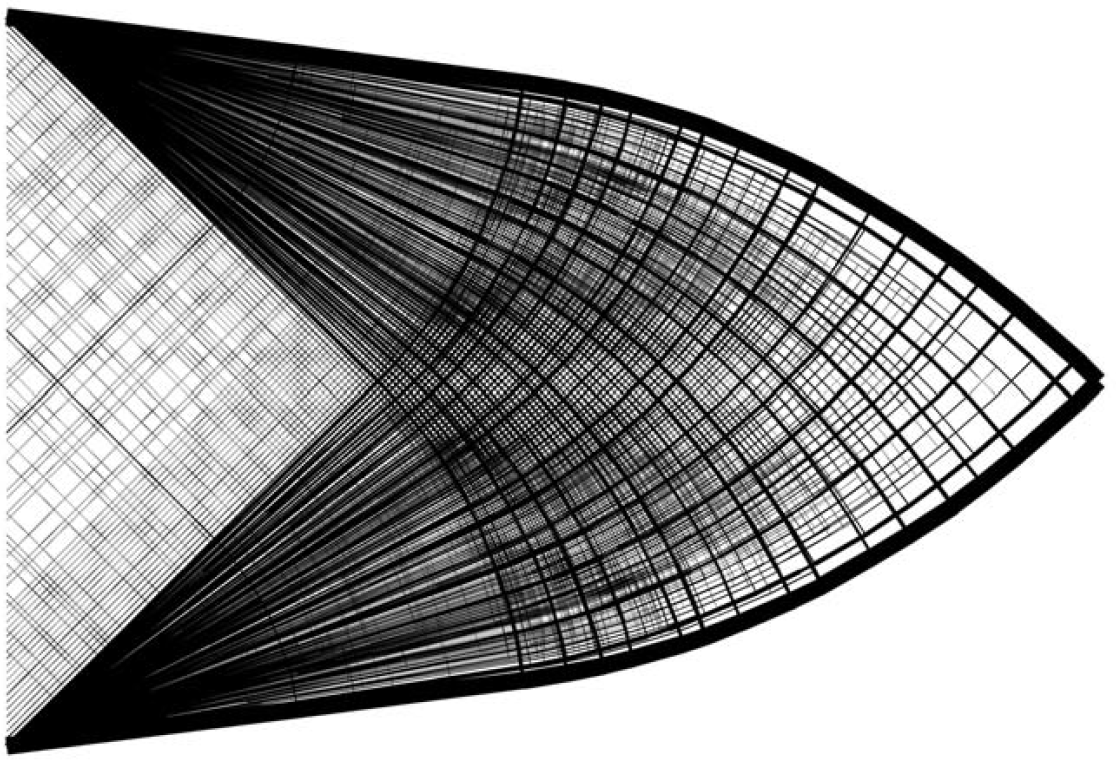
\includegraphics[width=\linewidth]{figures/03_comparison_TO_TTO/truss-ex.png}
    \caption{The optimal structures found by layout optimization tend at Michell-like structures, made up of a very large number of infinitesimal struts \cite{gilbert_layout_2003}.}
    \label{fig:03_truss-ex}
\end{marginfigure}

\section{Comparison between continuous and truss discretization} \label{sec:03_comparison}
In the upcoming discussion, we will be comparing the optimized structures using discrete and continuous meshes. Our primary objective in this comparison is to gain a comprehensive understanding of the application limits inherent in these two structural discretization methods. If, indeed, we identify such limitations, the aim is to discern and define them. Such discussions have already been pointed out in the literature~\sidecite{bendsoe_optimal_1989, watts_simple_2019}, but they are usually only empirical considerations and not numerical analysis.

Since our interest is in ultralight structures, we are especially interested in comparing the results of both optimization methods when dealing with different volume fractions on a common load case. Since we can't directly control volume in our formulation, we will adjust the material properties to influence the volume fraction of the optimized structure. For this comparative analysis, we have selected three key performance metrics: the volume fraction $V_\text{f}=V/\Omega$, the structural compliance $C$, and the maximum material allowable $\sigma_L$. Among these, we classify stress limit as the active metric used to influence the optimization, while volume and compliance are the objective of the optimization and a passive metric, respectively. In addition to the aforementioned performance metrics, we will also track the execution time of the algorithms.

\subsection{Definition of a common test case}
\begin{figure}
    \centering
    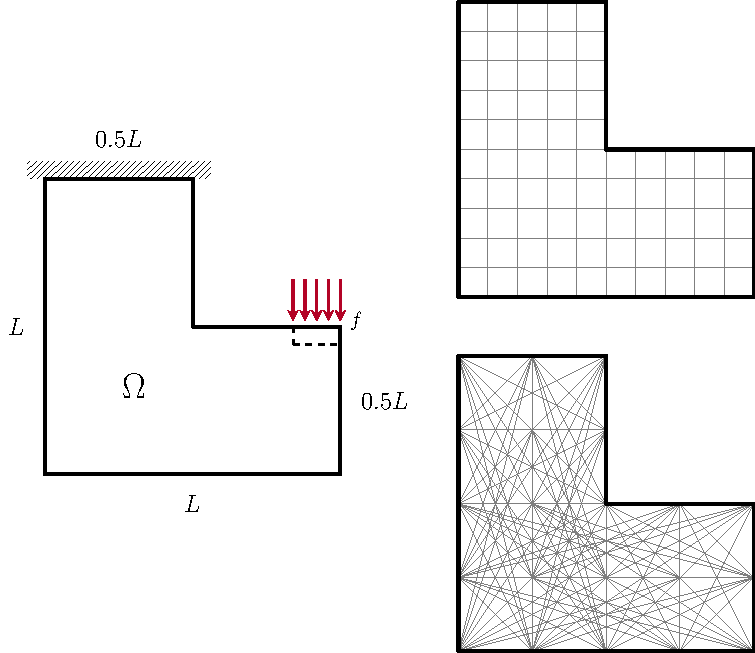
\includegraphics[scale=0.75]{figures/03_comparison_TO_TTO/06_L_bc/L_bc.pdf}
    \caption{On the left, plot of the L-shape beam test case, on the right the graphical representations of the two discretizations used, the continuous (above) and the truss-like (below).}
    \label{fig:03_L_bc}
\end{figure}
The L-shape beam is one of the most used load case benchmarks for stress-based topology optimization~\sidecite{duysinx_topology_1998,le_stress-based_2010}. This choice is driven by the distinctive geometry of the problem, which generates a stress concentration, particularly at the sharp corner—a phenomenon approaching infinity. Consequently, optimized solutions often feature a large fillet, mitigating the intensity of the stress singularity. The geometric description of the test case is given in \figref{fig:03_L_bc}. The beam with dimensions $L\times L$ presents an encastre on the top part and a load on the right extremity. For the continuous mesh case the load is distributed over multiple elements (5\% of $L$) to avoid stress concentrations and the stress constraints are not evaluated there. This zone is considered outside of the design domain $\Omega$.

To permit the discretization comparison, the structure is divided into two distinct meshes: in the continuous case, we employ a mesh consisting of $600\times600$ quadrilateral elements, totaling \num[group-separator={$\,$}]{270000} elements, while for the truss configuration, we employ a mesh with $33\times 33$ nodes and a fully connected ground structure, comprising a total of \num[group-separator={$\,$}]{305728} candidates.

We employ the same isotropic material and structure dimensions for the two optimizations, and the complete data is resumed in \tabref{tab:03_mat}. The value of the maximum material admissible $\sigma_\text{L}$ is used as the parameter that influences the volume fraction of the solutions. For simplicity, all numeric values are assumed normalized and dimensionless.

\begin{margintable}
    \small
    \centering
    \begin{tabular}{cc}
    \toprule
    \textbf{Parameter}        & \textbf{Value} \\ \midrule
    $E$              & 1     \\
    $\nu$            & 0.3   \\
    $L$              & 100   \\
    $\sigma_\text{L}$ & var. \\
    \bottomrule
    \end{tabular}
    \caption{Material data used for the optimizations. The value of the maximum material admissible $\sigma_\text{L}$ is used as the parameter to generate multiple optimized topologies.}
    \label{tab:03_mat}
\end{margintable}

\subsection{Numerical application} \label{sec:03_applications}
The focus of this section is to provide the numerical framework used to carry out the comparative analysis of the optimization results obtained from continuous and truss discretizations. The optimization formulations previously described have been implemented using Python.

The optimizing algorithm chosen for the continuous mesh is the \gls{mma}~\sidecite{svanberg_method_1987}. The parameter called \textit{movelimit}\sidenote{More information on the implementation of the \textit{movelimit} parameter can be found on the paper by Verbart \cite{verbart_unified_2017}} is set to $0.1$ while the other algorithm's parameters are set to their default value. A continuation scheme for the aggressiveness of the projection parameter $\beta$ is set to increase by one every 200 iterations, the number of max iteration is set to 7500, the stopping criteria is calculated as $\Vert r_k \Vert_2 / \sqrt{N_\text{e}}$ on the physical densities $\rhophys$ \cite{ferrari_new_2020}, and it is set to $10^{-4}$. The aggregation parameter $P$ of the aggregation function $G_{\text{KS}}^\text{L}$ is set to 32. The numerical implementation is carried out using the NLopt Python optimization framework~\sidecite{NLopt_2007}, analytically evaluating the sensitivity using \eqsref{eq:03_01} and \eqrefnotext{eq:03_sens-2}.

Formulation \ref{eq:03_optim_original} represents a \gls{lp} problem that can be efficiently solved by modern algorithms. In this work, we used the Python package CVXPY 1.2.2~\sidecite{diamond_cvxpy_2016} with the ECOS 2.0.7~\sidecite{domahidi_ecos_2013} solver. The joint cost $s$ is set to 0.001 and the stopping criteria is chosen as $\norm{\Delta \vect{x}}_\infty \leq 10^{-8}$. As Formulation is linear, no sensitivity calculation is carried out.

The optimizations presented in this section are performed on a server equipped with an Intel® Xeon® CPU E5-2650 @ \qty{2.20}{GHz} and using \qty{8}{GB} of RAM.

\paragraph{Coninuous mesh optimization results}
\begin{figure*}
    \subcaptionbox{}{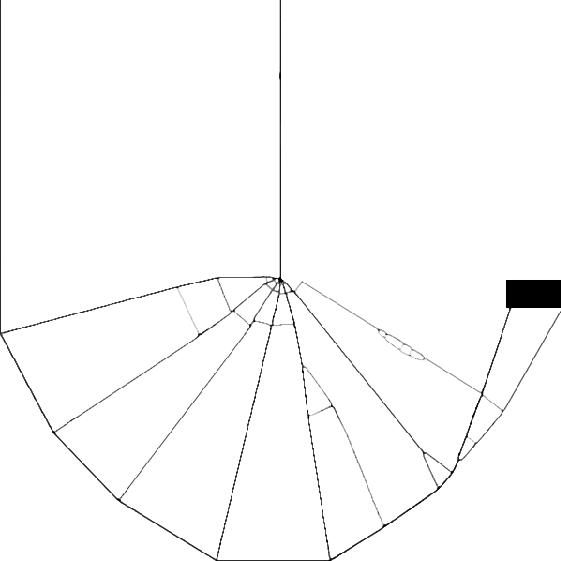
\includegraphics[width=0.23\linewidth ]{figures/03_comparison_TO_TTO/07_to_sol/fig0_10.pdf}}
    \hfill
    \subcaptionbox{}{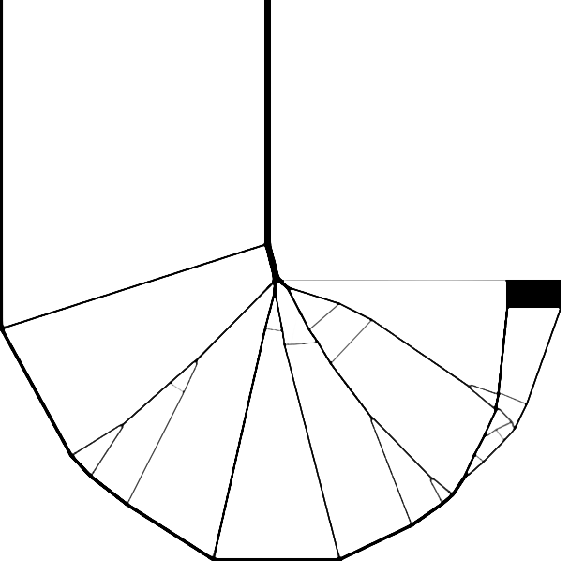
\includegraphics[width=0.23\linewidth ]{figures/03_comparison_TO_TTO/07_to_sol/fig0_2.pdf}}
    \hfill
    \subcaptionbox{}{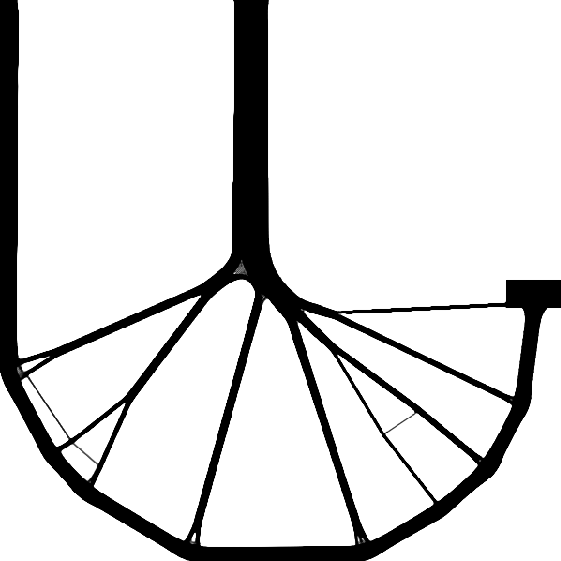
\includegraphics[width=0.23\linewidth ]{figures/03_comparison_TO_TTO/07_to_sol/fig0_0.4.pdf}}
    \hfill
    \subcaptionbox{}{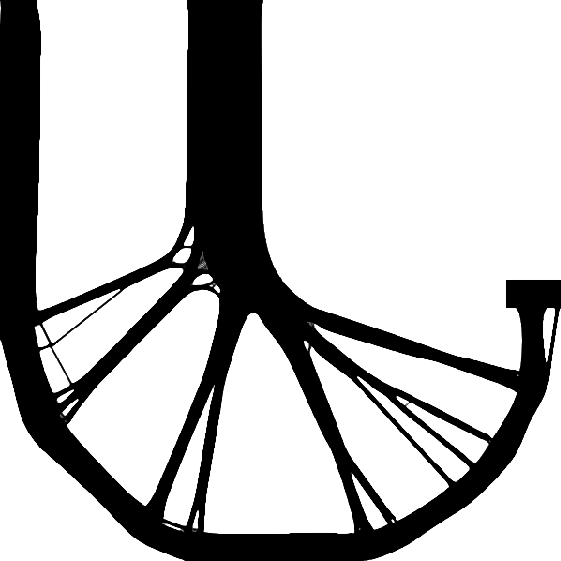
\includegraphics[width=0.23\linewidth ]{figures/03_comparison_TO_TTO/07_to_sol/fig0_0.25.pdf}}
    \bigskip
    \subcaptionbox{}{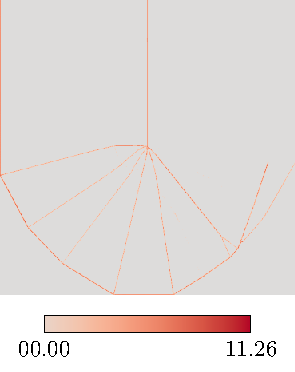
\includegraphics[width=0.23\linewidth ]{figures/03_comparison_TO_TTO/07_to_sol/stress_10.pdf}}
    \hfill
    \subcaptionbox{}{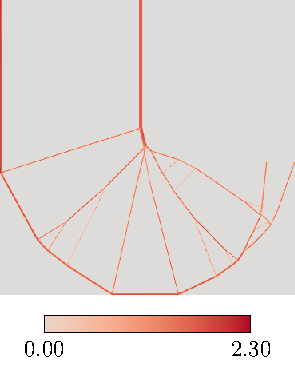
\includegraphics[width=0.23\linewidth ]{figures/03_comparison_TO_TTO/07_to_sol/stress_2.pdf}}
    \hfill
    \subcaptionbox{}{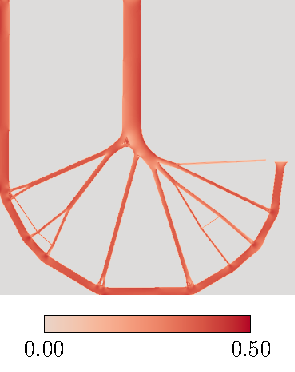
\includegraphics[width=0.23\linewidth ]{figures/03_comparison_TO_TTO/07_to_sol/stress_04.pdf}}
    \hfill
    \subcaptionbox{}{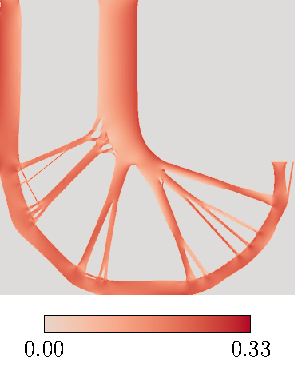
\includegraphics[width=0.23\linewidth ]{figures/03_comparison_TO_TTO/07_to_sol/stress_025.pdf}}
    \caption{(a-d) topology optimized structures for different material admissibles $\sigma_\text{L}=10.00,2.00,0.40\text{ and }0.25$, showing a volume fraction of $V_\text{f}=1.60\%,4.04\%,18.03\%\text{ and }34.71\%$, respectively. (e-h) Von Mises stress distribution of the optimized structures.}
    \label{fig:03_to_sol}
\end{figure*}
In this section, we generate multiple optimized structures with different volume fractions $V_\text{f}$ by launching the optimization code for continuous mesh with different values of the material admissible $\sigma_\text{L}$ spanning from $0.2$ to $20$.

On top of volume fraction, compliance, and stress, we evaluate an additional metric specific to continuous meshes called the \textit{measure of non-discreteness}~\sidecite{sigmund_morphology-based_2007} to evaluate the quality of the solutions. It is defined as:
\begin{equation}
    M_\text{nd} = \frac{\sum_e 4 \rhophys_e(1-\rhophys_e)}{n} \times 100 \%,
\end{equation}
where results near zero mean a completely black-and-white design. 

The results obtained for $\sigma_\text{L}=10.00,2.00,0.40\text{ and }0.25$ are shown in \figref{fig:03_to_sol}. In the upper part of the figure (a-d), we see the topology of the optimized structures with an ascending volume fraction $V_\text{f}$. Interestingly, the topology of the solution remains almost unchanged, varying principally in the thickness of its members. We notice the classic large fillet around the corner that alleviates the stress concentration problem. As the volume decreases, the optimized structure tends to a solution that resembles Michell structures, with a reducing fillet radius. In those cases, we know that the topology optimization algorithm acts as a method for the layout of truss-like structures~\sidecite{bendsoe_generating_1988}. This effect is caused by the combination of different factors, such as the regularization filter, the mesh size, and the low volume fraction~\sidecite{sigmund_non-optimality_2016}. A summary of the numerical results is presented in \tabref{tab:TO_results}.

In the lower part of \figref{fig:03_to_sol} (e-f), we plot the equivalent Von Mises stress for every element of the solution with physical density $\rhophys>0.5$. Multiple interesting observations can be made. First, we notice that the stress distribution is almost uniform in the structure, and it tends to the value of the material admissible $\sigma_\text{L}$ -- \ie we approach a \textit{fully stressed} structure. Even if the geometric support of the theory is different, it looks like the topology-optimized structures follow the Michell criteria presented in \secref{sec:03_michell} for optimal truss structures. Furthermore, it is observed that the maximum stress exceeds the material admissible $\sigma_\text{L}$. Aggregation methods aim to estimate the maximum value of the stress constraint across a group of elements. However, these aggregation methods do not perfectly align with the exact maximum value, which is a recognized limitation. To address this challenge, multiple approaches have been proposed within the aggregation framework to accurately account for the true constraint value, like using a set of active stress constraints~\sidecite{bruggi_topology_2012}, several aggregation clusters~\sidecite{paris_block_2010} or rectifier functions~\sidecite{norato_maximum-rectifier-function_2022}.

Looking again at \tabref{tab:03_TO_results}, we notice that the optimization processes exhibit long execution times, especially when dealing with extreme cases like high-volume fractions. This effect is likely caused by the very fine mesh used to discretize the design domain $\Omega$, by the sensitivity calculation by means of the adjoint method, and by the increasing difficulty of satisfying the stress constraints.

\begin{table}
    \small
    \centering
    \sisetup{table-auto-round}
    \begin{tabular}{S[table-format = 2.2]
                    S[table-format = 2.2]
                    S[table-format = 2.2]
                    S[table-format = 5.0]
                    S[table-format = 1.2]
                    S[table-format = 4.0]
                    c
                    }
    \toprule
    $\bm \sigma_L$ & $\bm \max \bm \sigma_L$   & $\bm V_\text{f}$     & $\bm C$ & $M_\text{nd}$  & {\textbf{It.}}  & {\textbf{Time}}      \\ \midrule
    20    & 23.51 & 1.18\ppercent       & 6992.10    & \qty{1.91}{\percent} & 1142     & $\hms{08;11;00}$ \\
    10    & 11.26 & 1.60\ppercent       & 3837.08    & \qty{2.19}{\percent} & 1147     & $\hms{07;55;00}$ \\
    8     & 8.78  & 1.74\ppercent       & 2765.60    & \qty{1.95}{\percent} & 792      & $\hms{05;39;00}$ \\
    6     & 7.15  & 1.89\ppercent       & 2243.31    & \qty{1.81}{\percent} & 806      & $\hms{05;35;00}$ \\
    5     & 5.81  & 2.17\ppercent       & 1823.12    & \qty{1.81}{\percent} & 849      & $\hms{05;53;00}$ \\
    4     & 4.69  & 2.67\ppercent       & 1423.54    & \qty{2.02}{\percent} & 894      & $\hms{06;12;00}$ \\
    3     & 3.47  & 3.00\ppercent       & 1132.79    & \qty{1.64}{\percent} & 993      & $\hms{06;45;00}$ \\
    2     & 2.30  & 4.04\ppercent       & 781.48     & \qty{1.45}{\percent} & 1189     & $\hms{08;20;00}$ \\
    1     & 1.18  & 7.28\ppercent       & 403.53     & \qty{1.35}{\percent} & 1621     & $\hms{11;41;00}$ \\
    0.90  & 1.06  & 8.09\ppercent       & 364.80     & \qty{1.31}{\percent} & 1656     & $\hms{11;36;00}$ \\
    0.80  & 0.96  & 8.82\ppercent       & 331.95     & \qty{1.21}{\percent} & 1937     & $\hms{15;21;00}$ \\
    0.70  & 0.84  & 10.05 \ppercent    & 291.89     & \qty{1.09}{\percent} & 1827     & $\hms{13;21;00}$ \\
    0.60  & 0.73  & 11.80 \ppercent    & 250.23     & \qty{1.19}{\percent} & 1955     & $\hms{14;21;00}$ \\
    0.50  & 0.61  & 14.18 \ppercent    & 213.01     & \qty{1.06}{\percent} & 2032     & $\hms{15;39;00}$ \\
    0.40  & 0.50   & 18.03\ppercent     & 169.90     & \qty{1.08}{\percent} & 2259     & $\hms{17;06;00}$ \\
    0.35  & 0.44  & 21.12 \ppercent    & 148.13     & \qty{1.15}{\percent} & 2421     & $\hms{19;29;00}$ \\
    0.30  & 0.38  & 26.21 \ppercent    & 125.69     & \qty{1.50}{\percent} & 3100     & $\hms{24;46;00}$ \\
    0.25  & 0.33  & 34.71 \ppercent    & 104.30     & \qty{1.04}{\percent} & 3484     & $\hms{27;39;00}$ \\
    0.20  & 0.27  & 48.08 \ppercent    & 76.56      & \qty{1.26}{\percent} & \color{accent_r_1}7500     & $\hms{91;46;00}$ \\ \bottomrule
    \end{tabular}
    \caption{Numerical results of the topology optimization method of the L-shape beam load case with varying material admissible $\sigma_\text{L}$ on a $600 \times 600$ elements mesh.}
    \label{tab:03_TO_results}
    \end{table}
    
\begin{marginfigure}
        \centering
        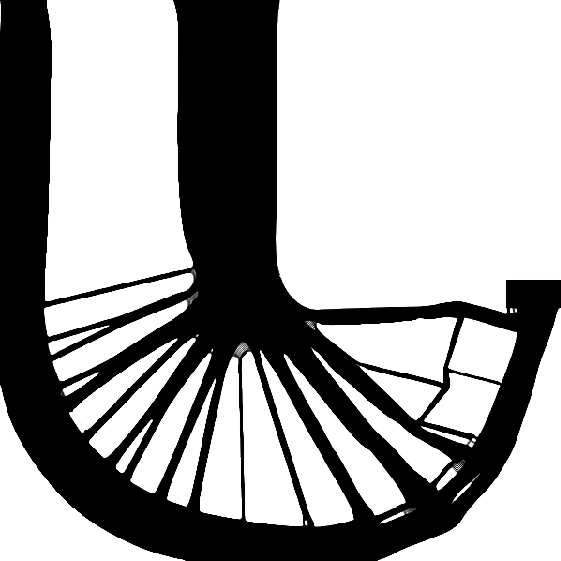
\includegraphics[width=0.8\linewidth]{figures/03_comparison_TO_TTO/08_to_no/fig0.pdf}
        \caption{The optimized structure for $\sigma_\text{L}=0.2$ with $V_\text{f}=\qty{48.08}{\percent}$, but does not converge after 7500 iterations.}
        \label{fig:03_to_sol_no}
    \end{marginfigure}

As previously mentioned, our focus lies in exploring the method's limits, particularly at the volume fraction boundaries. When dealing with excessively weak materials -- \ie materials that show a low $\sigma_\text{L}$, we encounter a scenario where no solution can be attained since no distribution can fulfill the imposed constraints. Throughout our research with this specific test case and mesh size, we did not produce any solutions with a volume fraction exceeding 50\%. Although we haven't reached that scenario with $\sigma_\text{L}$ set to 0.2, the calculation time and the number of iterations increase significantly,showing that we have encountered the method's limits. The calculation time has significantly increased because the algorithm faces greater difficulty in satisfying the stress constraints. \figref{fig:03_to_sol_no} shows the topology of the solution with $\sigma_\text{L}=0.2, \; V_\text{f}=\qty{48.08}{\percent}$ and over five days of optimization.

\begin{marginfigure}
    \centering
    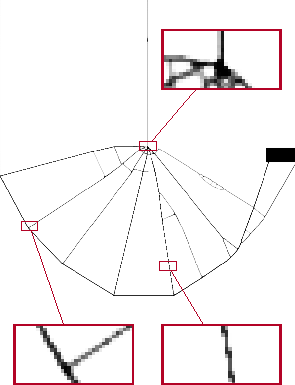
\includegraphics[width=0.8\linewidth]{figures/03_comparison_TO_TTO/09_to_zoom/to_zoom.pdf}
    \caption{The optimized structure for $\sigma_\text{L}=10.0$ with $V_\text{f}=\qty{1.60}{\percent}$. Some of the structure's features present not even a fully-dense element in their thickness.}
    \label{fig:03_to_sol_zoom}
\end{marginfigure}
Conversely, when dealing with exceedingly strong material -- \ie materials that show a high $\sigma_\text{L}$, the optimal scenario would demand such minimal material usage that certain sections of the structure become thinner than the width of a single element. In this case, the mesh used for discretization is too coarse to accurately represent the solution, and finer meshing becomes essential to capture the intricate details of the optimized design. \figref{fig:03_to_sol_zoom} shows
the limit case when $\sigma_\text{L}=10.0$ and $V_\text{f}=\qty{1.60}{\percent}$.

Finally, in \figref{fig:03_to_plot} are the plots summarizing our findings, with the limits highlighted. To effectively show the different orders of magnitude present in the plot, we have used both linear and logarithmic scales simultaneously.
\begin{figure*}
    \hspace*{\fill}
    \subcaptionbox{\label{fig:03_to_plot_lin}}{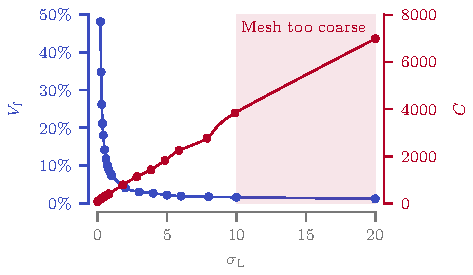
\includegraphics{figures/03_comparison_TO_TTO/10a_to_graph_lin/to_c_lin.pdf}}
    \hfill
    \subcaptionbox{\label{fig:03_to_plot_log}}{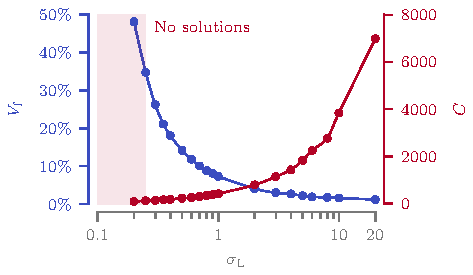
\includegraphics{figures/03_comparison_TO_TTO/10b_to_graph_log/to_c.pdf}}
    \hspace*{\fill}
    \caption{Linear (a) and logarithmic (b) plot of the volume fraction $V_\text{f}$ and the compliance $C$ with respect to the maximum material admissible $\sigma_\text{L}$ for the continuous mesh structures. Areas in red represent the boundaries of the applied method.}
    \label{fig:03_to_plot}
\end{figure*}
It's interesting to note that the volume fraction $V_\text{f}$ follows a hyperbolic relationship, while compliance $C$ exhibits a linear correlation with respect to the material admissible $\sigma_\text{L}$.

\paragraph{Truss mesh optimization results}
In this section, we present the optimized structures of the truss discretization. \figref{fig:03_L_tto} provides a visual representation of the topology and the corresponding stress distribution. Due to the inherent linearity properties of Formulation \ref{eq:03_optim_original}, several intriguing characteristics emerge. Notably, in the case of the tested L-shaped case, we encounter a scenario where the boundary conditions are neither overconstrained nor subject to asymmetric stress constraints. Consequently, this test case aligns with the Michell criteria. As a result, the topology does not vary regardless of the imposed stress limit, and the structure is fully stressed.
\begin{figure}
    \centering
    \hspace*{\fill}
    \subcaptionbox{\label{fig:03_tto_sol_tc}}{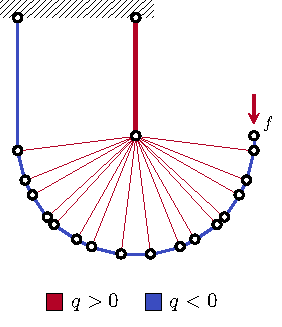
\includegraphics{figures/03_comparison_TO_TTO/11_tto_sol/L_tto_opt.pdf}}
    \hfill
    \subcaptionbox{\label{fig:03_tto_sol_st}}{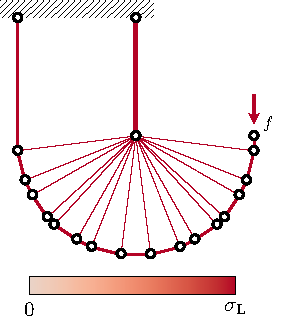
\includegraphics{figures/03_comparison_TO_TTO/11_tto_sol/L_tto_opt_st.pdf}}
    \hspace*{\fill}
    \caption{Topology (a) and stress (b) plot for the truss-like discretization.}
    \label{fig:03_L_tto}
\end{figure}
Additionally, the following equation consistently holds:
\begin{equation} \label{eq:03_V_star}
    V^*=\frac{fL}{\sigma_\text{L}}\cdot \text{const.},
\end{equation}
where the multiplicative constant depends on the load case and the ground structure used to discretize the design space $\Omega$ \sidecite{lewinski_extended_1994}. The execution time of the optimization is approximately \qty{90}{\second} and does not change with respect to the maximum stress $\sigma_\text{L}$. The results of the multiple optimizations can be found in \tabref{tab:03_TTO_results}.

\begin{table}
    \small
    \centering
    \sisetup{table-auto-round}
    \begin{tabular}{S[table-format = 2.1]
                    S[table-format = 2.2]
                    S[table-format = 5.0]
                    S[table-format = 2.1]                    
                    S[table-format = 2.0]}
        
    \toprule
    $\bm \sigma_L$ & $\bm V_\text{f}$     & $\bm C$      & {\textbf{Min} $\bm \lambda$} & {\textbf{Time}} \\ \midrule
    50         & 0.124169\ppercent  & 23281.62 & 111.687                     & $\hms{00;01;06}$    \\
    20         & 0.310422\ppercent  & 9312.65  & 70.637                      & $\hms{00;01;09}$    \\
    10         & 0.620843\ppercent  & 4656.32  & 49.948                      & $\hms{00;01;18}$    \\
    8          & 0.776054\ppercent  & 3725.06  & 44.675                      & $\hms{00;01;15}$    \\
    6          & 1.034739\ppercent  & 2793.79  & 38.689                      & $\hms{00;01;10}$    \\
    5          & 1.241686\ppercent  & 2328.16  & 35.318                      & $\hms{00;01;24}$    \\
    4          & 1.552108\ppercent  & 1862.53  & 31.590                      & $\hms{00;01;18}$    \\
    3          & 2.069477\ppercent  & 1396.90  & 27.358                      & $\hms{00;01;15}$    \\
    2          & 3.104216\ppercent  & 931.26   & 22.337                      & $\hms{00;01;15}$    \\
    1          & 6.208431\ppercent  & 465.63   & 15.795                      & $\hms{00;01;17}$    \\
    0.90       & 6.898257\ppercent  & 419.07   & 14.984                      & $\hms{00;01;20}$    \\
    0.80       & 7.760539\ppercent  & 372.51   & \color{accent_r_1}14.127    & $\hms{00;01;21}$    \\
    0.70       & 8.869187\ppercent  & 325.94   & \color{accent_r_1}13.215    & $\hms{00;01;16}$    \\
    0.60       & 10.347385 & 279.38\ppercent   & \color{accent_r_1}12.235    & $\hms{00;01;20}$    \\
    0.50       & 12.416862 & 232.82\ppercent   & \color{accent_r_1}11.169    & $\hms{00;01;22}$    \\
    \bottomrule    
    \end{tabular}
    \caption{Numerical results of the \gls{tto} method of the L-shape beam load case with varying material admissible $\sigma_\text{L}$ on a $33 \times 33$ ground structure.}
    \label{tab:03_TTO_results}
    \end{table}

    \begin{marginfigure}
        \centering
        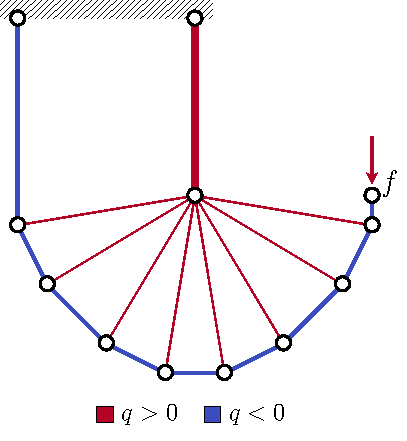
\includegraphics[width=0.8\linewidth]{figures/03_comparison_TO_TTO/12_tto_sol_13/L_tto_opt.pdf}
        \caption{Optimized structure obtained a fully connected ground structure with $13 \times 13$ and \num[group-separator={$\,$}]{7705} candidates.}
        \label{fig:03_L_tto_13}
    \end{marginfigure}
It's worth noting that we have intentionally opted for a fine mesh here to achieve a design variable count roughly equivalent to that of the continuous mesh case. We have utilized a fully connected ground structure with $33 \times 33$ nodes, but in reality, we obtain satisfactory results even with just $13 \times 13$ nodes (see \figref{fig:03_L_tto_13}). In this case we obtain a normalized volume $V^*=4.705 \; fL/\sigma_\text{L}$, signifying a \qty{1.05}{\percent} increase compared to the $33 \times 33$ case with $V^*=4.656 \; fL/\sigma_\text{L}$ with a variable count reduction of \qty{97.4}{\percent} (\num[group-separator={$\,$}]{305728} vs \num[group-separator={$\,$}]{7705} candidates). The computational time remains below one second.

In assessing solution quality, we employ a distinct metric known as the slenderness ratio, denoted as $\lambda$, which represents the ratio between the length and the radius of gyration of the bar. In our specific case, we have established a minimum slenderness ratio of 15. For a bar with a circular cross-sectional area, this corresponds to a radius of $R_\lambda$ for a bar length of $7.5\;R_\lambda$. We higlighted in red the optimized structures that does not repect the minimum slenderness ratio in \tabref{tab:03_TTO_results}. It is important to note that this metric is very sensible to the ground structure used: for example in the $13\times13$ nodes test case, $\lambda$ becomes critical ($\lambda=14.8$) only when $\sigma_\text{L}=0.25$ and $V_\text{f}=25.09$, suggesting that a control of this parameter during the optimization should be beneficial.

Lastly, \figref{fig:03_tto_plot} provides a visual summary of our findings, emphasizing in red the observed limits. To effectively show the different orders of magnitude present in the plot and how already done for the continuous mesh case, we have used both linear and logarithmic scales simultaneously. In this case, the compliance exhibits a perfectly linear relationship, while the volume follows a hyperbolic law in accordance with \eqref{eq:03_V_star}.

\begin{figure*}
    \hspace*{\fill}
    \subcaptionbox{\label{fig:03_tto_plot_lin}}{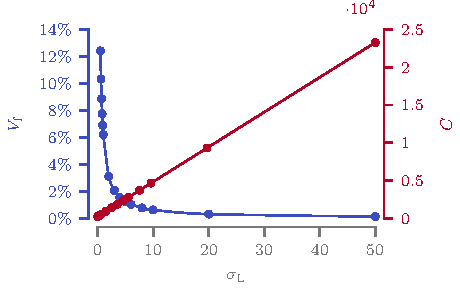
\includegraphics{figures/03_comparison_TO_TTO/13a_tto_graph_lin/tto_c_lin.pdf}}
    \hfill
    \subcaptionbox{\label{fig:03_tto_plot_log}}{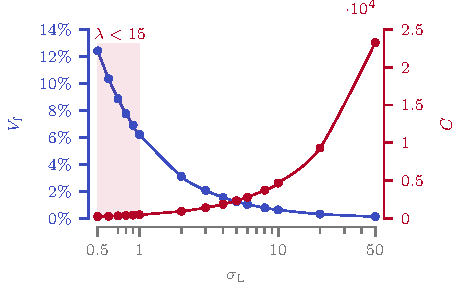
\includegraphics{figures/03_comparison_TO_TTO/13b_tto_graph_log/tto_c.pdf}}
    \hspace*{\fill}
    \caption{Linear (a) and logarithmic (b) plot of the volume fraction $V_\text{f}$ and the compliance $C$ with respect to the maximum material admissible $\sigma_\text{L}$ for the truss-like structures. Areas in red represent the boundaries of the applied method.}
    \label{fig:03_tto_plot}
\end{figure*}

\subsection{Discussion}
In this section, we present a series of graphs for the two formulations comparing the three figures of merit that have been considered thus far: the maximum material admissible $\sigma_\text{L}$, the compliance $C$, and the volume fraction $V_\text{f}$. It's important to note that the data presented in these graphs excludes the values that fall outside the limits highlighted for the two different discretizations in the previous subsections.
\begin{figure}
    \centering
    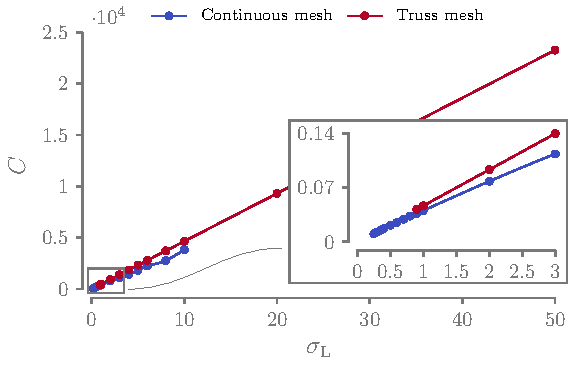
\includegraphics{figures/03_comparison_TO_TTO/14_stress_comp/stress_comp.pdf}
    \caption{Compliance -- Maximum material admissible plot for the continuous and truss discretizations.}
    \label{fig:03_stress_comp}
\end{figure}

\figref{fig:03_stress_comp} depicts the stress compliance graph for the L-shaped beam load case under consideration. It is evident that the truss configuration consistently exhibits lower compliance values for every considered material admissible and maintains a perfectly linear relationship, in contrast to the continuous discretization approach. We speculate that the difference may be attributed to the non-linearity of the formulation, potentially causing the continuous approach to converge to a local minimum.

In \figref{fig:03_stress_vol} we plot the different volume fractions obtained for a given material admissible (the axis in the graph are swapped as for us the most important figure of merit is the volume fraction).
\begin{figure}
    \centering
    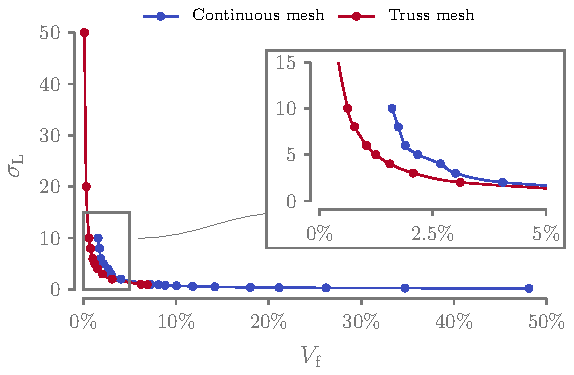
\includegraphics{figures/03_comparison_TO_TTO/15_stress_vol/stress_vol.pdf}
    \caption{Maximum material admissible -- Volume fraction plot for the continuous and truss discretizations.}
    \label{fig:03_stress_vol}
\end{figure}
The continuous mesh yields structures that are more massive for a given material limit. This outcome can be attributed not only to the aforementioned non-linearity in the formulation but also to another intriguing phenomenon. When dealing with volumes exceeding \qty{1}{\percent} (see \figref{fig:03_to_sol}b), we observe that the material in the topology-optimized structure is distributed across multiple elements, appearing somewhat “smeared”. In contrast, the truss representation concentrates all the structural mass along an imaginary line extending from one node to another, being more efficient.

We can also distinctly observe that the truss representation serves as the lower limit of the topology optimization for low volume fractions. Interestingly, both discretizations follow a similar trend for high-volume fractions, despite the significant disparity in their physical description models. The very same trends can be observed watching the volume-complaince graph of \figref{fig:03_comp_vol}.
\begin{figure}
    \centering
    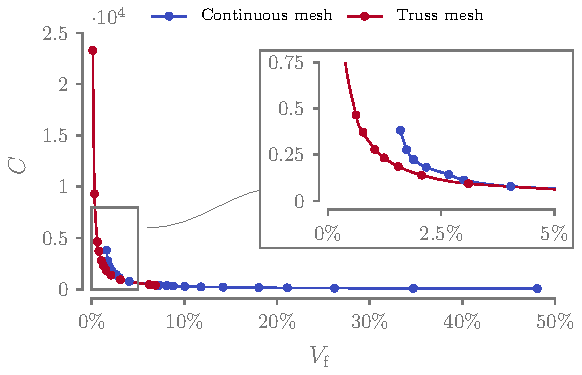
\includegraphics{figures/03_comparison_TO_TTO/16_comp_vol/comp_vol.pdf}
    \caption{Compliance -- Volume fraction plot for the continuous and truss discretizations.}
    \label{fig:03_comp_vol}
\end{figure}

Finally, in \figref{fig:03_time_vol} we turn our attention to the time comparison between the two optimization methods. It is noteworthy that a consistent three-order of magnitude difference is observed between the two methods (days vs. minutes). Additionally, it's worth recalling that in the truss case, employing an extremely fine ground structure is not a necessity, which implies that the time difference could potentially be even bigger.

\begin{figure}
    \centering
    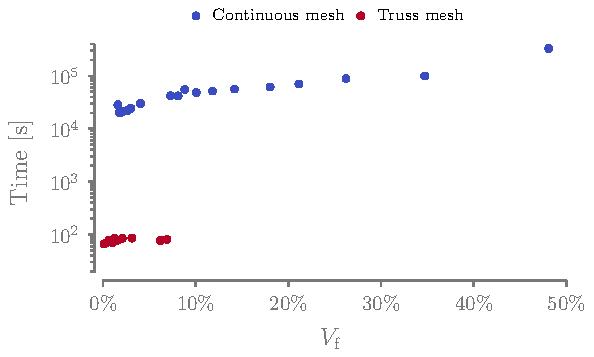
\includegraphics{figures/03_comparison_TO_TTO/17_time_vol/time_vol.pdf}
    \caption{Time -- Volume fraction plot for the continuous and truss discretizations.}
    \label{fig:03_time_vol}
\end{figure}

The notable difference in computation time for stress-based topology optimization (which is not self-adjoint in contrast to compliance minimization) points to the potential for exploring \gls{sand} topology optimization. While preliminary studies in this direction have been conducted~\sidecite{munro_local_2017}, they lie beyond the scope of this thesis and will not be further investigated. It's worth mentioning that \gls{sand} approaches typically lead to a substantial increase in the number of design variables. However, in truss topology problems, this is less of a concern due to the ground structure approach, which results in numerous cross-sectional area design variables and fewer displacement-related ones. This, however, does not hold when dealing with a continuous mesh.

To sum up, in comparing truss and continuous discretization methods, the advantages of truss structures become evident when considering the limitations of continuous discretization for the optimization of ultralight structures. One key drawback of continuous discretization is its increasing need for more elements as the desired level of refinement becomes finer at low volume fractions. Additionally, continuous discretization faces challenges with stress limits in optimized structures, which often exceed the specified admissible limits. Strategies exist to address this issue, but they come at the cost of increased computation time. Furthermore, stress constraints in continuous discretization are often defined for equivalent Von Mises stress, making it more challenging to distinguish between asymmetric bounds for tension and compression. Finally, truss structures are naturally subject to local buckling as a mode of failure~\sidecite{sigmund_non-optimality_2016}, a phenomenon that can be more easily and directly modeled in a truss discretization. 

While truss discretization offers advantages in terms of computational efficiency, it does come with certain limitations. In the minimum volume formulation, the problem is linear and cost-effective to solve. However, the linearity is lost when additional constraints, such as local buckling, are introduced. Moreover, the formulation does not inherently account for the kinematic compatibility of the problem. This limitation restricts its applicability to relatively simple problems and can pose issues when dealing with complex scenarios involving multiple loads or constraints that may lead to structures that are statically indeterminate.

Despite these challenges, we decided to favor truss discretization for our research. In the upcoming chapter, we will address and explore potential solutions to address its main limitations to further enhance its applicability and effectiveness.

\section{Conclusion}
Since the first developments of the topology optimization method, it has been recognized that "For moderately low volume fractions the lay-out of truss-like structures is predicted, but for very low volume fractions it is recommended that the traditional lay-out theory be employed..."~\sidecite{bendsoe_optimal_1989}. However, the performance gap has never been quantified, nor has the domain of applicability been assessed. This is the primary motivation behind this chapter. Additionally, it's important to note that these assumptions were primarily based on compliance formulations and not on volume minimization formulations, which are more pertinent to the aeronautical context.

In this chapter, we introduced a volume minimization formulation applicable to both continuous and truss-like discretizations, aiming at a meaningful comparison. We established a standardized two-dimensional test case, the L-shaped beam, commonly used in stress-based optimization. We conducted multiple optimization runs for both discretization methods using various materials and subsequently compared the results, focusing primarily on volume fraction, compliance, and stress in the optimized structures.

Considering the limitations encountered with the continuous approach, particularly at very low volume fractions, we opted for the truss discretization method for our specific research problem. We also identified certain limitations inherent to truss discretizations, which will be addressed in the following chapter.